% appendix_b
\chapter{Extension of an Empirically Driven Variability-Based Filtering Framework to Breast Tissue}
\label{app:empirical_variability_extension}

%-----------------------------------------------------------------------
\section{Motivation and Scope}
%-----------------------------------------------------------------------

The variability-based filtering strategy embedded in the preprocessing 
pipeline of this thesis builds directly on the method proposed 
by \cite{Edgar2017}, who demonstrated that a substantial fraction 
of CpG sites interrogated by the Illumina HumanMethylation450K array 
are effectively non-variable within a given tissue context and can 
therefore be removed prior to downstream analysis without loss of 
discriminative information. The original study was conducted on three 
healthy reference tissues — blood, buccal epithelial cells, and 
placenta — and the resulting non-variable CpG lists were shown to be 
robust across preprocessing pipelines and normalisation strategies.

The present appendix documents the extension of this framework to 
breast tissue. The extension pursues two objectives: (i) to assess 
whether the non-variability criterion, as originally defined, 
generalises to a cancer-relevant tissue under increased biological 
heterogeneity; and (ii) to provide a general, reproducible protocol 
for incorporating additional tissues into the reference framework 
in future studies. The analysis operates exclusively on 
histologically normal samples to preserve comparability with the 
original reference tissues and to estimate baseline methylation 
stability in the absence of disease-related confounding.
Importantly, this appendix does not modify the non-variability 
definition of \cite{Edgar2017}: a CpG is classified as non-variable 
if its inter-quantile range $r_{\beta,j} = Q_{0.90}(\beta_j) - 
Q_{0.10}(\beta_j) < 0.05$. The contribution is therefore evaluative and integrative rather than definitional.

%-----------------------------------------------------------------------
\section{General Framework for Cross-Tissue Extension}
\label{app:sec:framework}
%-----------------------------------------------------------------------

Let $\mathcal{T} = \{T_1, \dots, T_k\}$ denote a set of reference 
tissues, each represented by one or more independent methylation 
datasets from normal samples. For each tissue $T_\ell$, the 
tissue-specific non-variable CpG set is defined as:
\begin{equation}
    \mathcal{N}_\ell(\tau)
    =
    \left\{
    j \in \{1,\dots,p\} :
    Q_{0.90}\!\left(\beta_j^{(\ell)}\right)
    -
    Q_{0.10}\!\left(\beta_j^{(\ell)}\right)
    < \tau
    \right\},
    \label{eq:nv_tissue}
\end{equation}
where $\tau = 0.05$ is the threshold inherited from 
\cite{Edgar2017}. The cross-tissue invariant core — CpGs 
non-variable across all reference tissues simultaneously — is 
given by the intersection:
\begin{equation}
    \mathcal{N}_{\mathrm{core}}(\tau)
    =
    \bigcap_{\ell=1}^{k} \mathcal{N}_\ell(\tau).
    \label{eq:nv_core}
\end{equation}
When a new tissue $T_{k+1}$ is incorporated, the invariant 
core is updated as:
\begin{equation}
    \mathcal{N}_{\mathrm{core}}'(\tau)
    =
    \mathcal{N}_{\mathrm{core}}(\tau)
    \;\cap\;
    \mathcal{N}_{k+1}(\tau),
    \label{eq:nv_update}
\end{equation}
which is strictly more conservative than the original core: 
$\mathcal{N}_{\mathrm{core}}'(\tau) \subseteq 
\mathcal{N}_{\mathrm{core}}(\tau)$.
The validation of any extension requires verifying three 
properties before the updated core can be considered 
methodologically sound.
\begin{enumerate}
    \item \textbf{Selection stability}: the non-variable set 
    $\mathcal{N}_{k+1}(\tau)$ must be robust to dataset 
    composition, i.e.\ not driven by any single cohort 
    (Step~A, Section~\ref{app:sec:stepA}).
    \item \textbf{Threshold optimality}: the chosen $\tau$ 
    must lie at a favourable stability--dimensionality 
    trade-off point in the new tissue context 
    (Step~B, Section~\ref{app:sec:stepB}).
    \item \textbf{Empirical coherence}: the selected CpGs 
    must exhibit methylation and variability profiles 
    consistent with the non-variability interpretation, 
    ruling out selection artefacts 
    (Steps~C--D, Sections~\ref{app:sec:stepC}--\ref{app:sec:stepD}).
\end{enumerate}
This three-step validation protocol is general and applies 
identically to any future tissue extension.

%-----------------------------------------------------------------------
\section{Cross-Tissue Overlap Structure}
\label{app:sec:overlap}
%-----------------------------------------------------------------------

Breast tissue was introduced alongside the three original 
reference tissues of \cite{Edgar2017}. Figure~\ref{fig:point0_global_structure} 
reports the overlap structure of tissue-specific non-variable 
CpG sets across all four tissues.
The four-way invariant core $\mathcal{N}_{\mathrm{core}}'(0.05)$ 
comprises 29,989 CpGs — a substantial shared subset whose 
persistence despite the inclusion of a cancer-relevant tissue 
suggests that at least a component of CpG non-variability reflects stable, context-independent properties of the methylation 
landscape rather than purely tissue-specific regulatory 
programmes. The breast-exclusive non-variable set (5,023 CpGs) 
is the smallest tissue-specific component, consistent with the 
expectation that breast tissue introduces additional 
heterogeneity relative to the original healthy tissue panel.
\begin{figure}[t]
\centering
\begin{subfigure}[t]{0.48\textwidth}
  \centering
  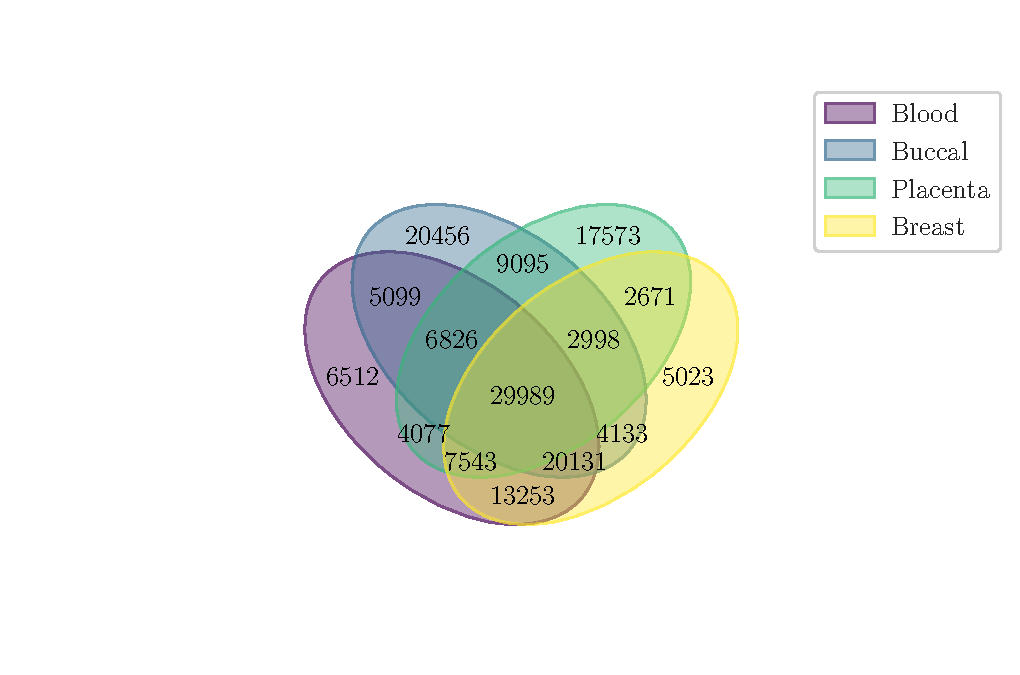
\includegraphics[width=\textwidth]{images/appendix/venn_4tissues_invariants.pdf}
  \caption{Pairwise and higher-order overlaps of tissue-specific 
  non-variable CpG sets.}
\end{subfigure}
\hfill
\begin{subfigure}[t]{0.48\textwidth}
  \centering
  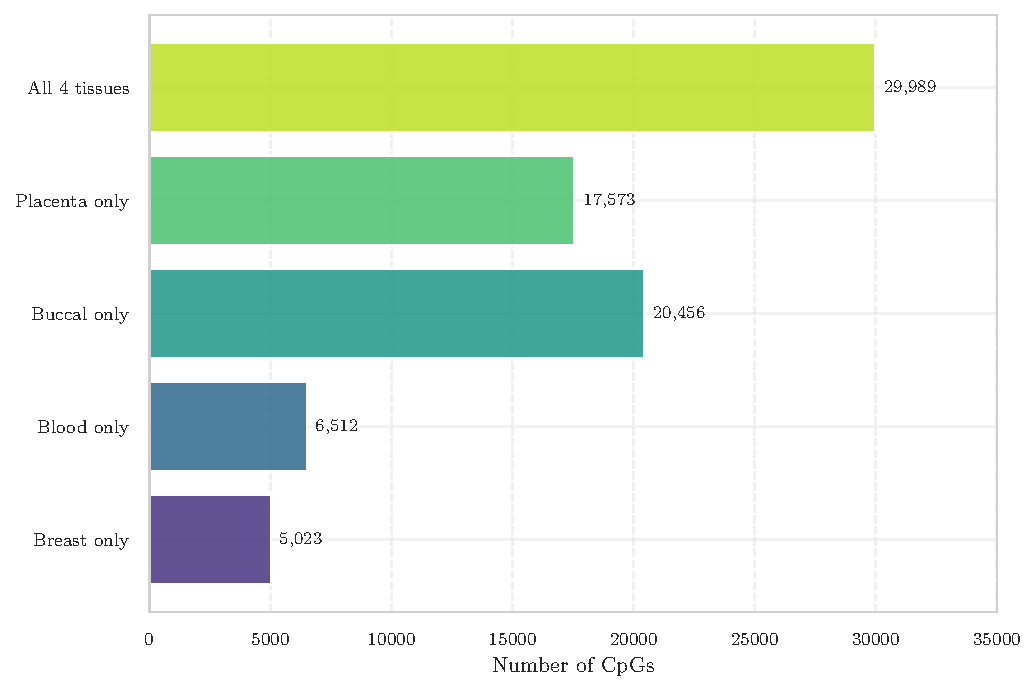
\includegraphics[width=\textwidth]{images/appendix/barplot_key_intersections_invariants.pdf}
  \caption{Quantitative intersection sizes for key subsets.}
\end{subfigure}
\caption{Global overlap structure of non-variable CpGs across 
blood, buccal epithelial cells, placenta, and breast tissue. 
}
\label{fig:point0_global_structure}
\end{figure}


%-----------------------------------------------------------------------
\subsection{Step A: Stability of Non-Variable CpG Selection}
\label{app:sec:stepA}
%-----------------------------------------------------------------------

The first validation step assesses whether the breast-tissue 
non-variable set $\mathcal{N}_{\mathrm{breast}}(\tau)$ is 
robust to dataset composition. A leave-one-dataset-out (LODO) 
strategy is adopted: for each held-out dataset 
$\mathcal{D}^{(-s)}$, the non-variable set is recomputed on 
the remaining datasets and compared to the full-reference set 
via the retention rate:
\begin{equation}
    \rho^{(-s)}
    =
    \frac{
        \left|\mathcal{N}_{\mathrm{breast}}^{(-s)}(\tau)
        \cap
        \mathcal{N}_{\mathrm{breast}}(\tau)\right|
    }{
        \left|\mathcal{N}_{\mathrm{breast}}(\tau)\right|
    },
    \label{eq:retention}
\end{equation}
where $\mathcal{N}_{\mathrm{breast}}^{(-s)}(\tau)$ denotes 
the non-variable set estimated without dataset $s$.
\begin{figure}[t]
\centering
\begin{subfigure}[t]{0.48\textwidth}
  \centering
  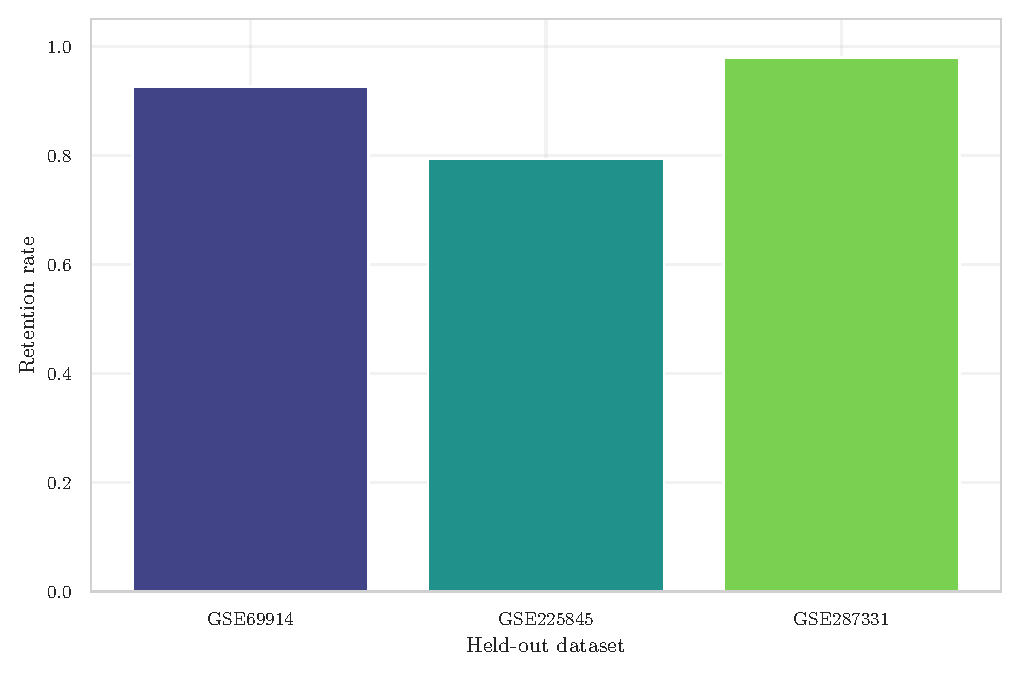
\includegraphics[width=\textwidth]{images/appendix/stepA_lodo_stability.pdf}
  \caption{Retention rates under the LODO protocol across 
held-out datasets (GSE69914, GSE225845, GSE287331).}
  \label{fig:stepA_lodo}
\end{subfigure}
\hfill
\begin{subfigure}[t]{0.48\textwidth}
  \centering
  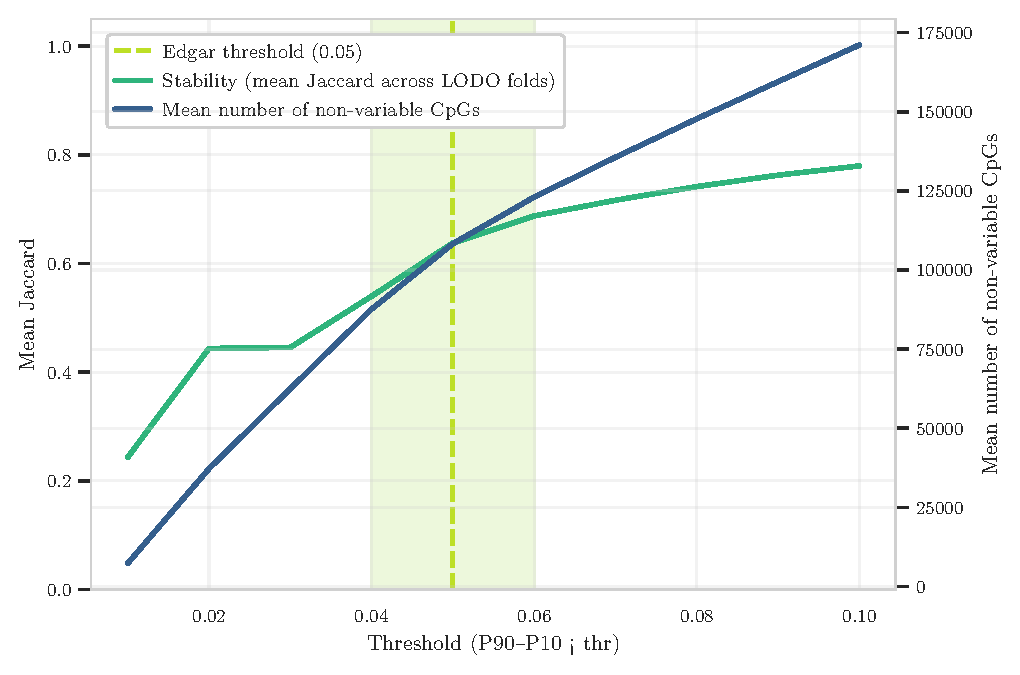
\includegraphics[width=\textwidth]{images/appendix/stepB_stability_vs_list_size_highlighted.pdf}
  \caption{Mean Jaccard similarity $J(\tau)$ and mean 
non-variable CpG count as functions of the threshold.}
  \label{fig:stepB_stability_vs_size}
\end{subfigure}

\caption{Assessment of robustness and trade-off between stability and dimensionality of non-variable CpG sets.}
\label{fig:stepAB}
\end{figure}
The retention rates reported in Figure~\ref{fig:stepA_lodo} 
are consistently high across all three held-out datasets, 
demonstrating that $\mathcal{N}_{\mathrm{breast}}(\tau)$ 
is not an artefact of any individual cohort but reflects 
a stable property of the underlying methylation variability 
structure in breast tissue. This result satisfies the first 
validation criterion stated in Section~\ref{app:sec:framework} 
and is a necessary condition for interpreting non-variability 
as a genuine empirical property rather than a dataset-specific 
anomaly.

%-----------------------------------------------------------------------
\subsection{Step B: Stability--Dimensionality Trade-Off}
\label{app:sec:stepB}
%-----------------------------------------------------------------------

Having established stability at $\tau = 0.05$, Step~B 
evaluates whether this threshold represents an optimal 
compromise between selection reproducibility and 
dimensionality reduction in the breast tissue setting. 
The mean Jaccard similarity across LODO folds and the 
mean number of non-variable CpGs are computed as 
functions of $\tau \in [0.01, 0.10]$:
\begin{equation}
    J(\tau)
    =
    \frac{1}{S}
    \sum_{s=1}^{S}
    \frac{
        \left|\mathcal{N}_{\mathrm{breast}}^{(-s)}(\tau)
        \cap
        \mathcal{N}_{\mathrm{breast}}(\tau)\right|
    }{
        \left|\mathcal{N}_{\mathrm{breast}}^{(-s)}(\tau)
        \cup
        \mathcal{N}_{\mathrm{breast}}(\tau)\right|
    }.
    \label{eq:jaccard}
\end{equation}
As shown in Figure~\ref{fig:stepB_stability_vs_size}, 
$J(\tau)$ increases rapidly for small $\tau$ and 
saturates before the Edgar threshold, while the CpG 
count continues to grow approximately linearly. 
At $\tau = 0.05$, stability is already at its 
near-maximum value and the marginal gain from 
increasing the threshold further is negligible relative 
to the dimensionality cost incurred. This empirically 
validates the original threshold of \cite{Edgar2017} 
in the breast tissue context and provides a 
data-driven justification for its retention within 
the extended framework.

%-----------------------------------------------------------------------
\subsection{Step C: Methylation Distribution of Non-Variable CpGs}
\label{app:sec:stepC}
%-----------------------------------------------------------------------

Step~C characterises the methylation profiles of the 
selected non-variable CpGs by comparing their 
$\beta$-value distribution to a random background 
sample of array CpGs, computed on normal breast 
samples pooled across datasets.
\begin{figure}[t]
\centering
\begin{subfigure}[t]{0.48\textwidth}
  \centering
  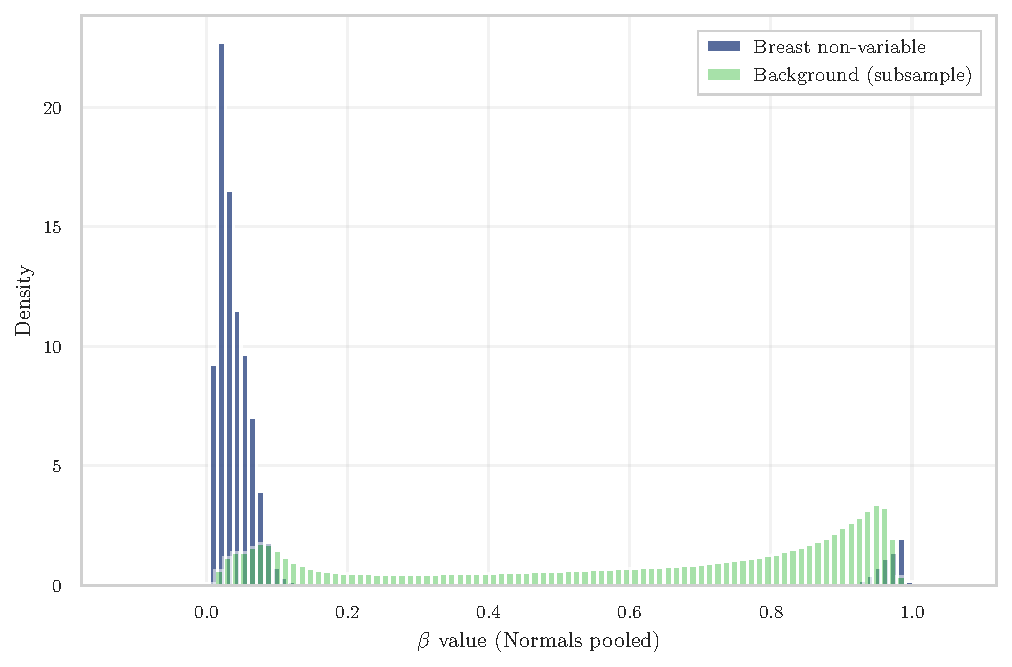
\includegraphics[width=\textwidth]{images/appendix/stepC_beta_distribution_nv_vs_background.pdf}
  \caption{Beta-value density for non-variable CpGs 
(breast tissue) versus genomic background.}
  \label{fig:stepC_beta_distribution}
\end{subfigure}
\hfill
\begin{subfigure}[t]{0.48\textwidth}
  \centering
  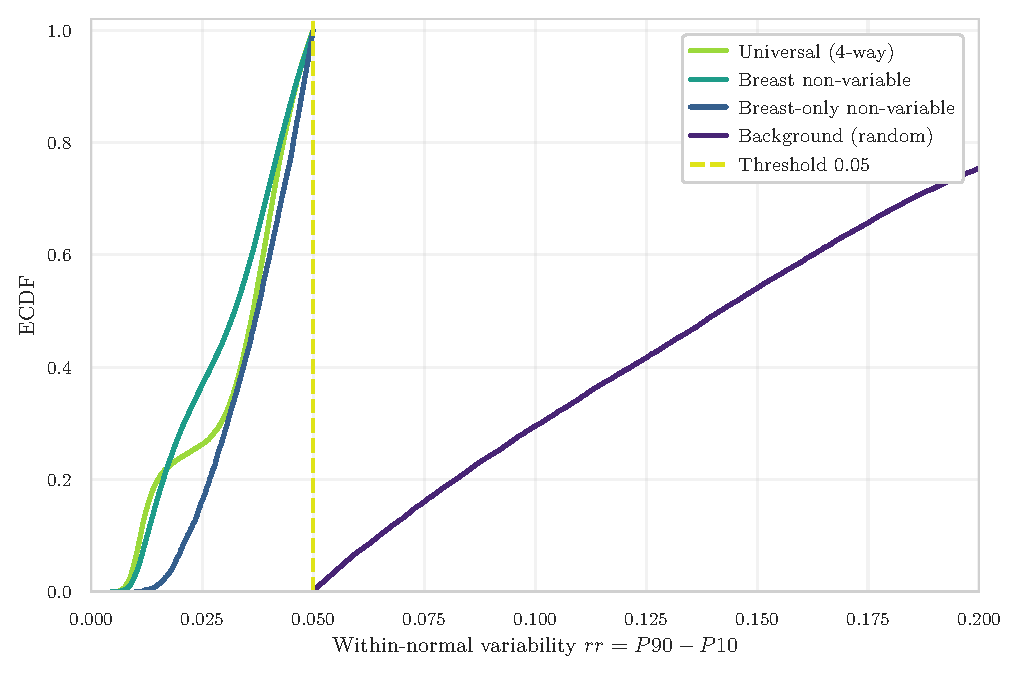
\includegraphics[width=\textwidth]{images/appendix/stepD_baseline_rr_ecdf.pdf}
  \caption{ECDF of within-normal variability 
$r_{\beta,j} = Q_{0.90} - Q_{0.10}$ across CpG subsets.}
  \label{fig:stepD_rr_ecdf}
\end{subfigure}

\caption{Characterization of the selected non-variable CpG set in terms of methylation distribution and baseline risk behavior.}
\label{fig:stepCD}
\end{figure}
Non-variable CpGs in breast tissue are strongly 
concentrated at extreme $\beta$ values, consistent 
with constitutive hypo- or hypermethylated states. 
This pattern replicates the findings of \cite{Edgar2017} 
in healthy tissues and extends them to a cancer-relevant 
context, supporting the interpretation that 
non-variability reflects stable regulatory configurations 
rather than artefacts of tissue composition or 
disease-related heterogeneity. The enrichment of 
non-variable CpGs in CpG islands and constitutively 
silenced promoter regions, documented in the original 
study, is consistent with this bimodal profile 
\cite{Edgar2017, Bock2012}.

%-----------------------------------------------------------------------
\subsection{Step D: Baseline Variability Profile}
\label{app:sec:stepD}
%-----------------------------------------------------------------------

Step~D provides quantitative validation of the filtering 
criterion by examining the empirical cumulative distribution 
function (ECDF) of $r_{\beta,j}$ across four CpG subsets: 
the four-way shared non-variable core 
$\mathcal{N}_{\mathrm{core}}'(0.05)$, the breast-specific 
non-variable set $\mathcal{N}_{\mathrm{breast}}(0.05)$, 
the breast-exclusive component, and a random background set.
The ECDFs in Figure~\ref{fig:stepD_rr_ecdf} show a 
clear separation: the non-variable subsets are sharply 
concentrated at low $r_{\beta,j}$ values, with the 
majority of CpGs well below $\tau = 0.05$, whereas 
the background distribution spans a substantially 
wider range. This confirms that the selected CpGs 
are empirically distinct in their variability profile 
and not merely defined as non-variable by construction. 
The consistency of this pattern across all non-variable 
subsets — including the breast-exclusive component — 
further supports the robustness of the extended 
framework.

%-----------------------------------------------------------------------
\section{Cohort-Resolved Characterisation of Breast-Tissue Non-Variability}
\label{app:sec:dataset_specific}
%-----------------------------------------------------------------------
The four-step validation protocol described in 
Section~\ref{app:sec:framework} establishes the methodological 
soundness of the non-variability criterion at the level of 
pooled breast data. The present section extends this 
characterisation to the individual-cohort level, pursuing two 
complementary objectives: (i) to assess whether the filtering 
behaviour is consistent across independent datasets, each with 
distinct sample compositions and phenotypic configurations; and 
(ii) to characterise the biological identity of the invariant CpG 
set through genomic contextual enrichment analysis and 
cross-phenotype variability concordance. Together, these analyses 
situate the breast-tissue extension within a broader biological 
framework and provide the empirical grounding required for its 
use as a preprocessing step in 
Chapter~\ref{chap:feature_selection}.

%-----------------------------------------------------------------------
\subsection{Empirical Variability Spectrum Across Independent Breast Cohorts}
\label{app:sec:empirical_variability_spectrum}
%-----------------------------------------------------------------------

To evaluate the consistency of the non-variability criterion across datasets, 
the inter-quantile range statistic 
$r_{\beta,j} = Q_{0.90}(\beta_j) - Q_{0.10}(\beta_j)$ 
was computed independently for each of the three breast cohorts 
(GSE69914, GSE225845, GSE287331). For each dataset, the analysis was 
carried out under two phenotypic configurations: 
(i) Normal + Adjacent (N+A), which includes only histologically normal 
and adjacent-normal samples, and (ii) Normal + Tumor (N+T), which 
additionally incorporates tumor samples. This design allows direct 
assessment of whether malignant tissue alters the global variability 
spectrum of CpG loci and, consequently, the proportion of sites 
classified as non-variable under the Edgar threshold 
$\tau = 0.05$.

Figure~\ref{fig:app_rbeta_distributions_all} reports the empirical density 
of $r_{\beta}$ under the N+T configuration for each dataset, with 
vertical markers indicating the three candidate thresholds 
$\tau \in \{0.01, 0.02, 0.05\}$. Several structural features are common 
to all three cohorts. The distribution is strongly right-skewed, with 
a pronounced mass concentrated near $r_{\beta} \approx 0$, indicating 
that a substantial fraction of CpG sites exhibit minimal within-group 
dispersion regardless of sample composition. The strict thresholds 
$\tau = 0.01$ and $\tau = 0.02$ remove only a small minority of loci, 
whereas the canonical $\tau = 0.05$ eliminates a sizeable but controlled 
proportion — 77,687 CpGs in GSE69914, 103,622 in GSE225845, and 
168,663 in GSE287331 — consistent with the dimensionality reduction 
reported in the pooled analysis.
A biologically informative pattern emerges from the comparison between 
the two phenotypic configurations. Under N+T, the Edgar filter removes 
fewer CpGs than under N+A: the greater methylation contrast between 
normal and tumor samples elevates $r_{\beta}$ across a larger fraction 
of loci, reducing the proportion that falls below $\tau = 0.05$. By 
contrast, the N+A configuration — whose analogous plots are reported in 
Chapter~\ref{chap:feature_selection} — yields a higher count of 
non-variable CpGs, reflecting the subtler methylation differences between 
histologically normal tissue and adjacent-normal samples. This asymmetry 
is consistent with the concept of field cancerization, whereby tissue 
adjacent to a tumour undergoes epigenetic alterations that, while not yet 
producing overt histological change, partially converge towards the tumour 
methylation profile. Under this interpretation, the reduced variability 
observed in N+A relative to N+T is not a statistical artefact but reflects 
a genuine biological phenomenon: adjacent tissue shares a greater proportion 
of its methylation landscape with normal tissue than tumor tissue does, 
resulting in a larger set of CpG sites that appear non-variable within the 
combined sample.

\begin{figure}[p]
    \centering

    % -------- (a) GSE69914 --------
    \begin{subfigure}{0.55\linewidth}
        \centering
        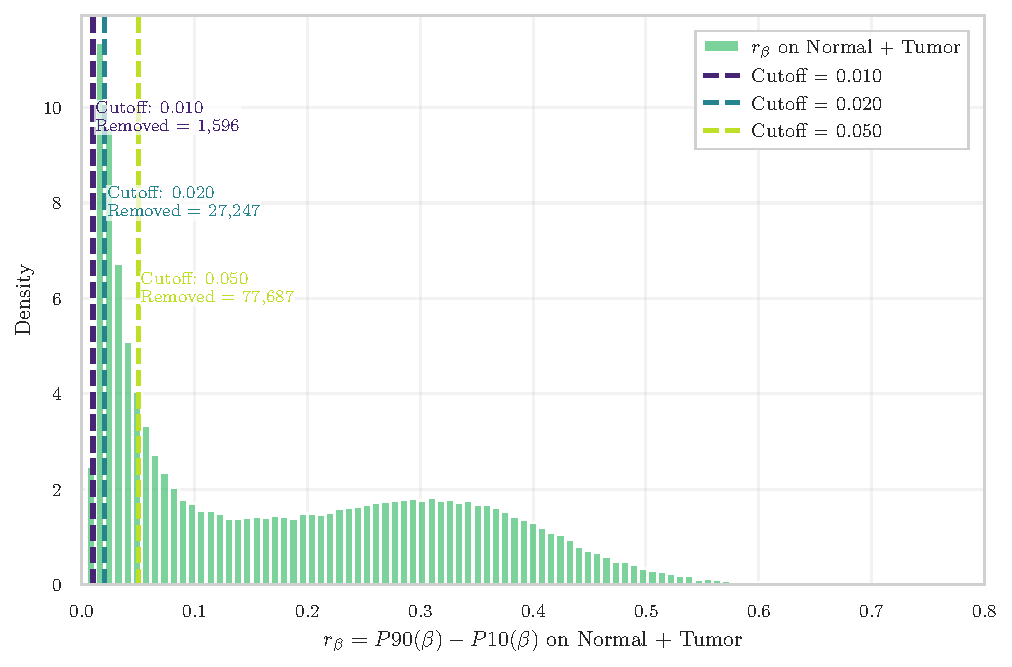
\includegraphics[width=\linewidth]{images/appendix/GSE69914_r_beta_distribution_NT_study}
        \caption{GSE69914}
        \label{fig:app_rbeta_dist_69914}
    \end{subfigure}

    \vspace{0.5cm}

    % -------- (b) GSE225845 --------
    \begin{subfigure}{0.55\linewidth}
        \centering
        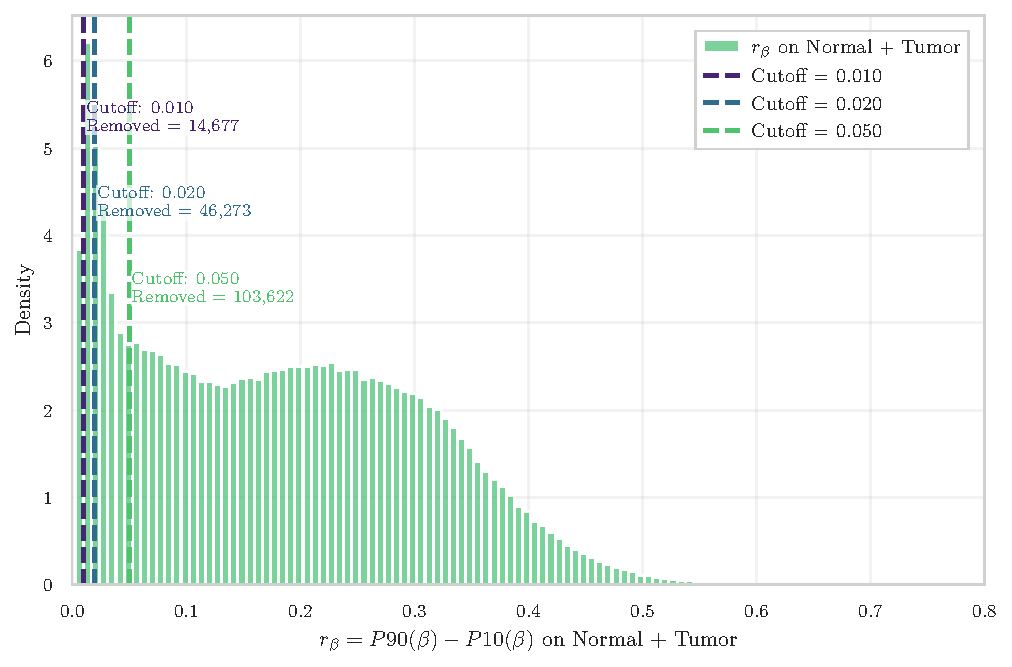
\includegraphics[width=\linewidth]{images/appendix/GSE225845_r_beta_distribution_NT_study}
        \caption{GSE225845}
        \label{fig:app_rbeta_dist_225845}
    \end{subfigure}

    \vspace{0.5cm}

    % -------- (c) GSE287331 --------
    \begin{subfigure}{0.55\linewidth}
        \centering
        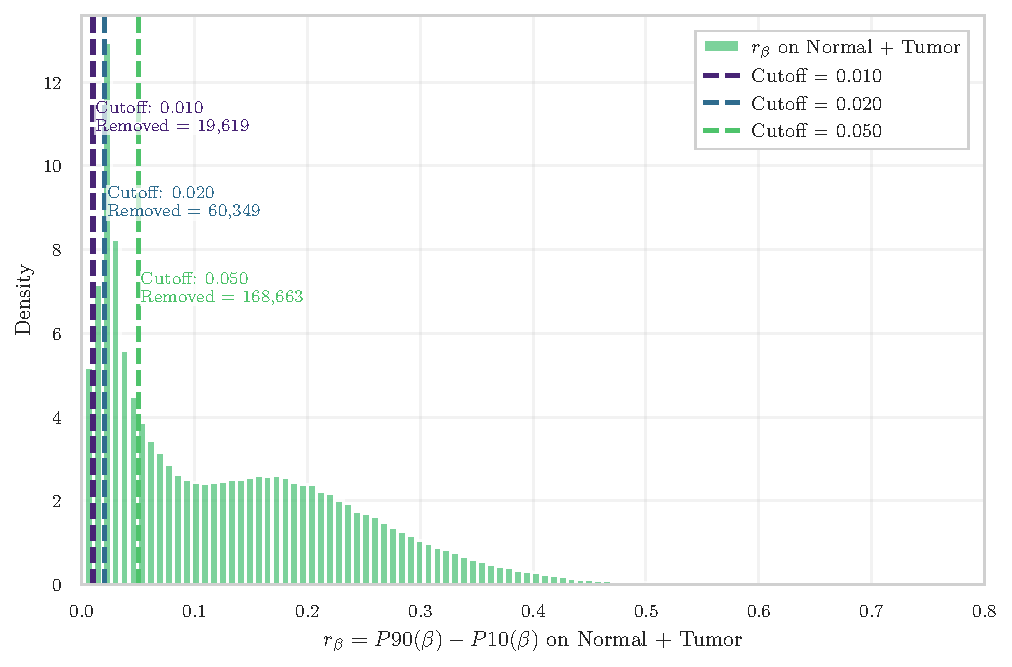
\includegraphics[width=\linewidth]{images/appendix/GSE287331_r_beta_distribution_NT_study}
        \caption{GSE287331}
        \label{fig:app_rbeta_dist_287331}
    \end{subfigure}

    \caption{
    Distribution of $r_{\beta}$ computed on the Normal+Tumor comparison for each dataset.
    Vertical dashed lines indicate the selected threshold.
    }
    \label{fig:app_rbeta_distributions_all}
\end{figure}

%-----------------------------------------------------------------------
\subsection{Contextual Enrichment Profile of Invariant CpGs}
%-----------------------------------------------------------------------

To characterise the genomic architecture of CpGs classified as 
non-variable under the Edgar threshold, a contextual enrichment 
analysis was performed using Illumina manifest annotations. 
Each probe was mapped to its corresponding gene-feature category 
(e.g., TSS200, TSS1500, 5'UTR, 1stExon, Body, 3'UTR, Intergenic), 
and enrichment was quantified as fold-change relative to the full 
set of interrogated CpGs within the dataset.
Let $\mathcal{U}$ denote the universe of CpGs and 
$\mathcal{N}_{\mathrm{breast}}(0.05)$ the invariant subset 
identified in the N+A configuration. For each annotation category 
$g$, enrichment was computed as:

\begin{equation}
  \text{FC}_g
=
\frac{
\frac{|\mathcal{N}_{\mathrm{breast}}(0.05) \cap g|}{|\mathcal{N}_{\mathrm{breast}}(0.05)|}
}{
\frac{|\mathcal{U} \cap g|}{|\mathcal{U}|}
}.
\end{equation}


Figure~\ref{fig:app_enrichment_all} reports the fold-change 
profile for the dominant gene-feature categories.
Across datasets, invariant CpGs show consistent enrichment in 
proximal promoter regions (particularly TSS200 and 1stExon) and 
relative depletion in gene bodies and distal regions. The baseline 
reference (fold-change = 1) indicates the expected frequency under 
random sampling from the array; deviations above this threshold 
reflect preferential localisation of low-variability CpGs within 
regulatory domains.
This pattern is coherent with the bimodal methylation behaviour 
described in Section~\ref{app:sec:stepC}, where invariant CpGs were 
shown to concentrate at constitutive hypo- or hypermethylated states. 
Promoter-associated CpG islands are known to exhibit tight regulatory 
control and reduced dispersion in normal tissue, providing a 
biologically plausible explanation for the observed enrichment.

Importantly, the enrichment structure is stable across cohorts, 
indicating that genomic localisation of invariant CpGs reflects 
intrinsic regulatory constraints rather than dataset-specific 
artefacts.


\begin{figure}[t]
    \centering

    % -------- (a) GSE69914 --------
    \begin{subfigure}[t]{0.31\linewidth}
        \centering
        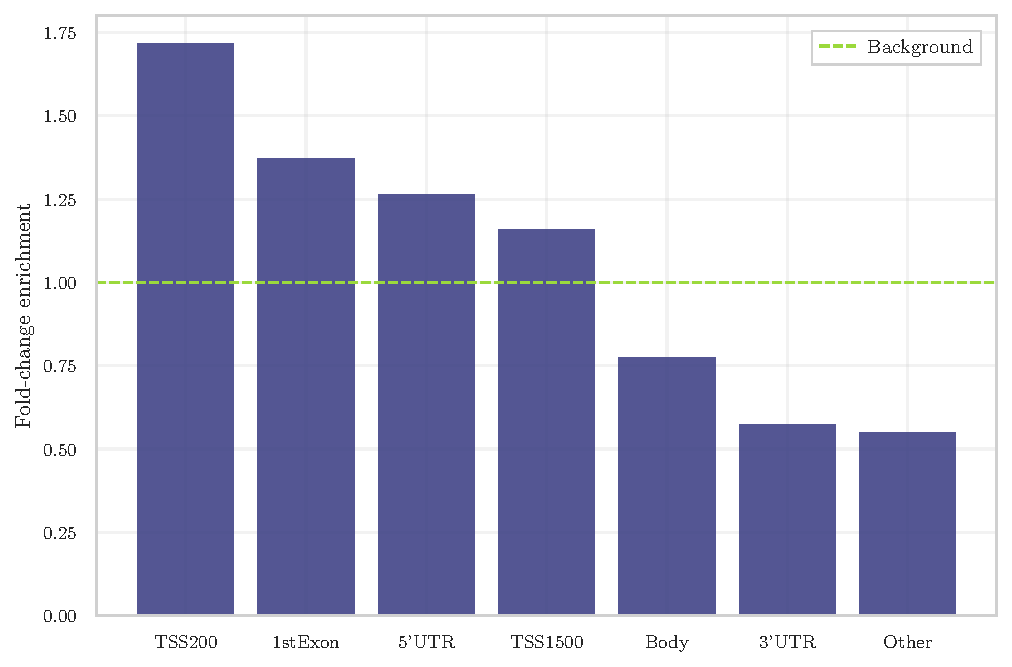
\includegraphics[width=\linewidth]{images/appendix/GSE69914_plot_enrichment_gene_invariant}
        \caption{GSE69914}
        \label{fig:app_enrichment_69914}
    \end{subfigure}
    \hfill
    % -------- (b) GSE225845 --------
    \begin{subfigure}[t]{0.31\linewidth}
        \centering
        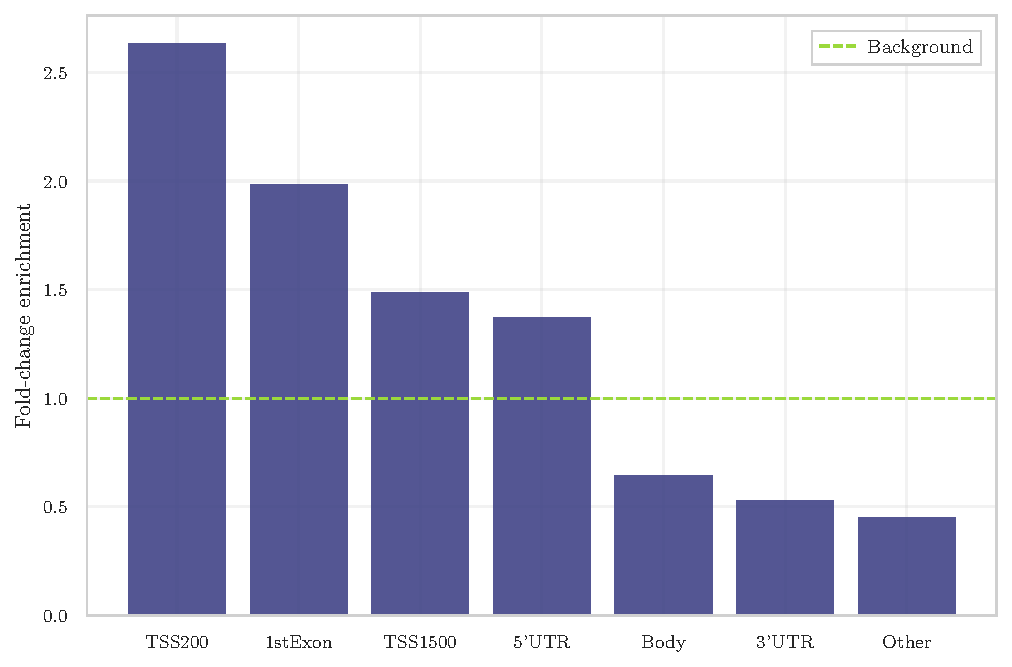
\includegraphics[width=\linewidth]{images/appendix/GSE225845_plot_enrichment_gene_invariant}
        \caption{GSE225845}
        \label{fig:app_enrichment_225845}
    \end{subfigure}
    \hfill
    % -------- (c) GSE287331 --------
    \begin{subfigure}[t]{0.31\linewidth}
        \centering
        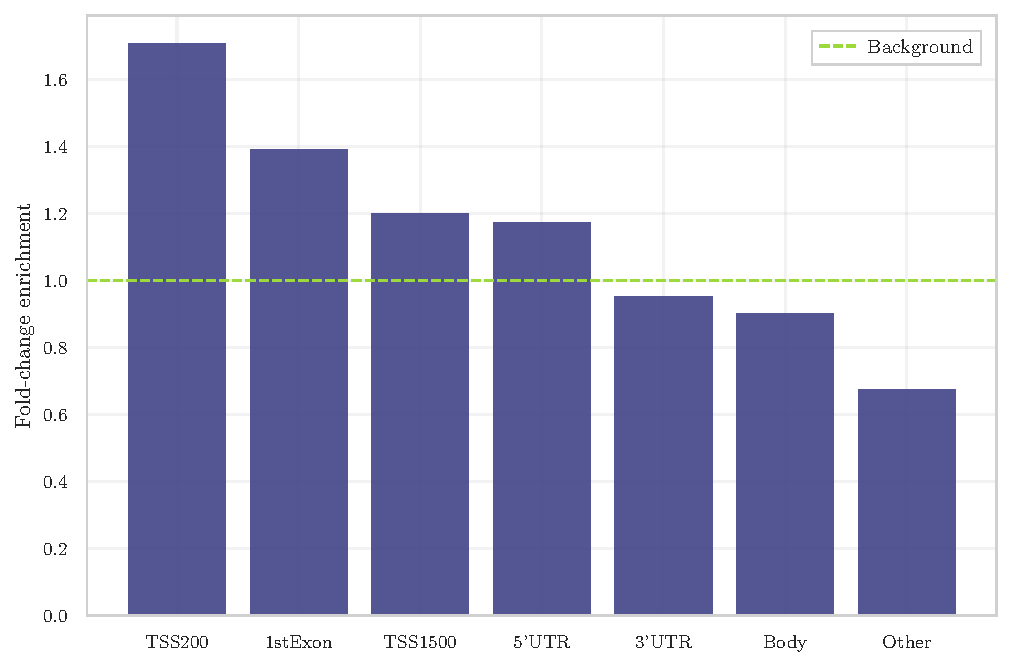
\includegraphics[width=\linewidth]{images/appendix/GSE287331_plot_enrichment_gene_invariant}
        \caption{GSE287331}
        \label{fig:app_enrichment_287331}
    \end{subfigure}

    \caption{
    Fold-enrichment of genomic context categories among invariant CpGs 
    relative to the background distribution in each dataset. 
    The dashed line indicates enrichment equal to background (fold = 1).
    }
    \label{fig:app_enrichment_all}
\end{figure}


%-----------------------------------------------------------------------
\subsection{Phenotype-Resolved Variability Concordance Analysis}
%-----------------------------------------------------------------------
\label{app:sec:phenotype_concordance}
Section~\ref{app:sec:empirical_variability_spectrum} established that 
the aggregate variability spectrum is qualitatively preserved when 
tumor samples are incorporated. The present section quantifies this 
concordance at the level of individual CpG sites by directly comparing 
$r_{\beta}$ values computed under the N+A and N+T configurations.
For each CpG $j$, the pair 
$\left(r_{\beta,j}^{(NA)}, r_{\beta,j}^{(NT)}\right)$ 
was examined and rank concordance was quantified via the Spearman 
correlation coefficient. Figure~\ref{fig:app_rbeta_scatter_all} 
displays the resulting scatter plots together with the identity line 
$y = x$ for each dataset. The Spearman coefficients are 
$\rho \approx 0.845$ (GSE69914), 
$\rho \approx 0.881$ (GSE225845), and 
$\rho \approx 0.933$ (GSE287331), 
indicating strong to very strong rank preservation of CpG-level 
variability across phenotypic configurations.
Several structural features emerge from the scatter plots. The bulk of 
CpG loci cluster tightly around the identity line, confirming that 
relative variability ordering is largely maintained when tumor samples 
are included. A minority of loci deviate upward from the diagonal, 
corresponding to CpGs whose dispersion increases in the presence of 
tumor tissue; by contrast, very few loci exhibit a systematic decrease 
in variability under N+T. This asymmetry is consistent with the 
expectation that malignant transformation introduces epigenetic 
heterogeneity rather than convergence, and corroborates the finding in 
Section~\ref{app:sec:empirical_variability_spectrum} that tumor 
inclusion primarily affects loci in the intermediate variability range.
The high rank concordance implies that the non-variability criterion is 
largely phenotype-robust: CpGs classified as low-variability under the 
N+A configuration remain predominantly low-variability when tumor 
samples are incorporated. This result supports the interpretation that 
breast-tissue non-variability reflects stable structural properties of 
methylation regulation, with tumor-associated heterogeneity manifesting 
as localised deviations superimposed on an otherwise preserved 
variability backbone.


\begin{figure}[t]
    \centering

    % -------- (a) GSE69914 --------
    \begin{subfigure}[t]{0.31\linewidth}
        \centering
        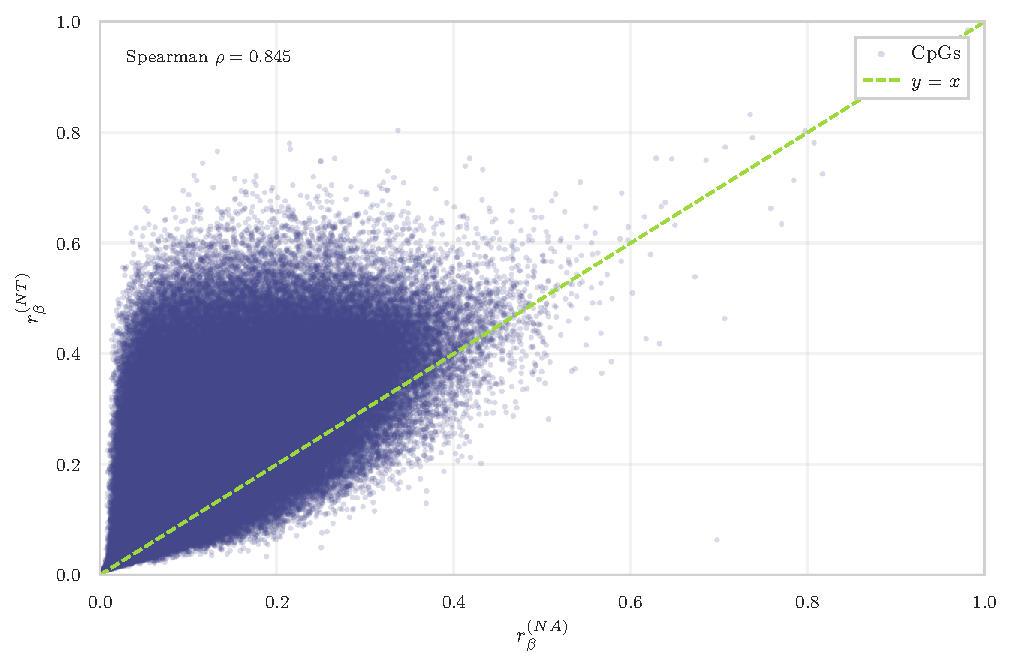
\includegraphics[width=\linewidth]{images/appendix/GSE69914_plot_scatter_rbeta_NA_vs_NT}
        \caption{GSE69914 \\ Spearman $\rho \approx 0.845$}
        \label{fig:app_rbeta_scatter_69914}
    \end{subfigure}
    \hfill
    % -------- (b) GSE225845 --------
    \begin{subfigure}[t]{0.31\linewidth}
        \centering
        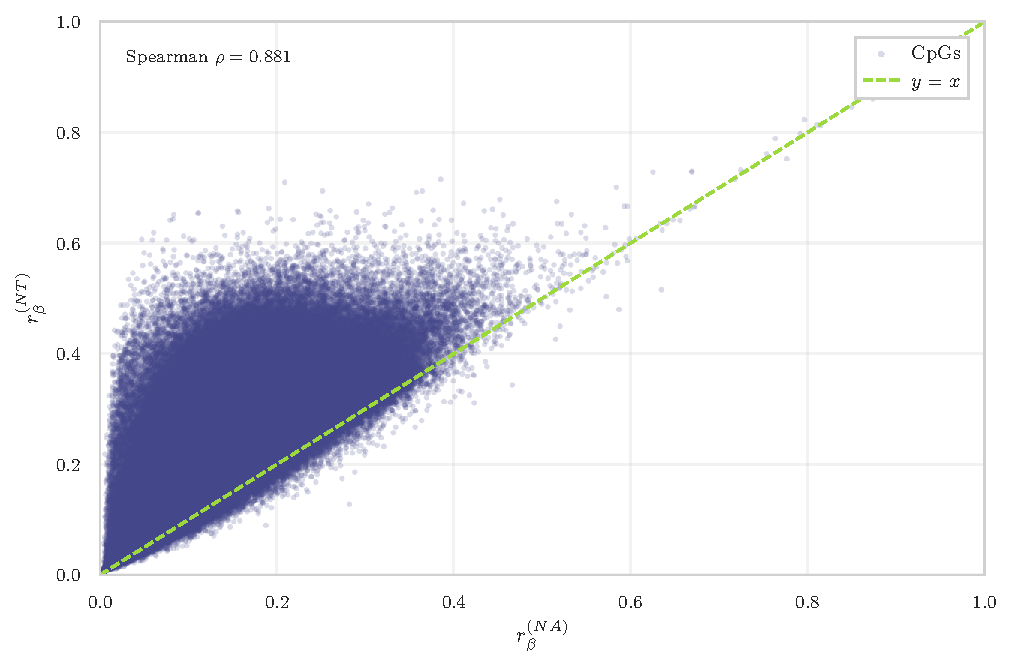
\includegraphics[width=\linewidth]{images/appendix/GSE225845_plot_scatter_rbeta_NA_vs_NT}
        \caption{GSE225845 \\ Spearman $\rho \approx 0.881$}
        \label{fig:app_rbeta_scatter_225845}
    \end{subfigure}
    \hfill
    % -------- (c) GSE287331 --------
    \begin{subfigure}[t]{0.31\linewidth}
        \centering
        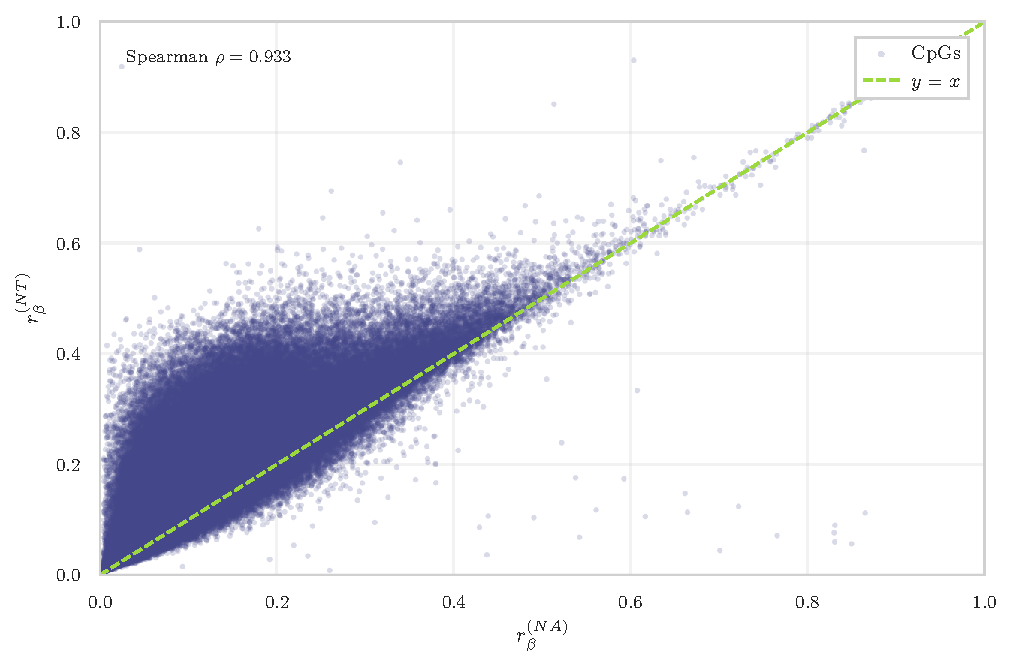
\includegraphics[width=\linewidth]{images/appendix/GSE287331_plot_scatter_rbeta_NA_vs_NT}
        \caption{GSE287331 \\ Spearman $\rho \approx 0.933$}
        \label{fig:app_rbeta_scatter_287331}
    \end{subfigure}

    \caption{
    Spearman correlation between CpG-level $\Delta\beta$ values 
    computed in the Normal+Adjacent and Normal+Tumor contrasts 
    for each dataset. The diagonal line represents identity.
    }
    \label{fig:app_rbeta_scatter_all}
\end{figure}

%-----------------------------------------------------------------------
\subsection{Invariant-Set Partitioning Across Phenotypic Combinations}
%-----------------------------------------------------------------------

The analyses in 
Sections~\ref{app:sec:empirical_variability_spectrum}–
\ref{app:sec:phenotype_concordance} establish that non-variability 
in breast tissue is broadly stable across both cohorts and 
phenotypic configurations. The present section integrates the 
breast-tissue invariance structure with the reference framework 
of~\cite{Edgar2017} by performing a set-theoretic decomposition 
that explicitly accounts for the effect of tumor inclusion.
Let 
\(
\mathcal{B}
=
\mathcal{N}_{\mathrm{Blood}}
\cap
\mathcal{N}_{\mathrm{Buccal}}
\cap
\mathcal{N}_{\mathrm{Placenta}}
\)
denote the universal invariant set across the three reference 
tissues of~\cite{Edgar2017}. The breast-tissue non-variable sets 
$\mathcal{N}_{\mathrm{breast}}(0.05)$ were estimated separately 
under the N+A and N+T configurations for each cohort. The 
intersection of $\mathcal{B}$ with these two sets defines three 
biologically interpretable invariant classes.

\paragraph{Core invariants
\(
\mathcal{B}
\cap
\mathcal{N}_{\mathrm{breast}}^{(NA)}(0.05)
\cap
\mathcal{N}_{\mathrm{breast}}^{(NT)}(0.05)
\)}
CpGs that are non-variable across all reference tissues and 
remain invariant in breast tissue irrespective of tumor 
inclusion. These loci constitute the most conserved component 
of the cross-tissue epigenetic backbone.

\paragraph{Conditionally variable universal CpGs
\(
\mathcal{B}
\cap
\mathcal{N}_{\mathrm{breast}}^{(NA)}(0.05)
\setminus
\mathcal{N}_{\mathrm{breast}}^{(NT)}(0.05)
\)}
Loci that are invariant across all reference tissues and in 
normal breast tissue but become variable when tumor samples 
are incorporated. This subset identifies CpGs whose stability 
is sensitive to malignant transformation and that may be of 
interest for cancer-specific methylation studies.

\paragraph{Breast-specific invariants
\(
\left(
\mathcal{N}_{\mathrm{breast}}^{(NA)}(0.05)
\cap
\mathcal{N}_{\mathrm{breast}}^{(NT)}(0.05)
\right)
\setminus
\mathcal{B}
\)}
CpGs that are consistently non-variable within breast tissue 
under both phenotypic configurations but are not part of the 
universal cross-tissue invariant core. These loci reflect 
tissue-contextual stability that is specific to breast 
epithelium.

Figure~\ref{fig:app_venn_universal_vs_breast} visualises this 
set-theoretic decomposition for each dataset as a three-way 
Venn diagram. The quantitative breakdown is consistent across 
cohorts. The core invariant class comprises approximately 
27,000–28,000 CpGs per dataset (GSE69914: 28{,}241; 
GSE225845: 26{,}542; GSE287331: 27{,}577), representing a highly 
conserved epigenetic backbone that is robust to both tissue 
context and phenotypic variation. The conditionally variable 
universal class is markedly smaller (GSE69914: 2{,}010; 
GSE225845: 1{,}353; GSE287331: 496), confirming that only a 
minor fraction of cross-tissue invariants is susceptible to 
tumor-induced destabilisation. The breast-specific invariant 
class is the largest component in datasets with denser sampling 
(GSE69914: 138{,}256; GSE225845: 76{,}223; GSE287331: 46{,}788), reflecting the greater 
CpG coverage of the corresponding platforms and the broader set 
of tissue-contextual constraints captured at higher array density.
Several biological observations emerge from this decomposition. 
First, the invariant core is not globally eroded by cancer: 
tumor-associated variability acts locally on a bounded subset of 
CpGs, while the structural invariance backbone is preserved. 
Second, the breast-specific invariant class is predominantly 
shared between the N+A and N+T configurations, confirming that 
tissue-contextual stability is itself phenotype-robust. Third, 
the hierarchical organisation of the invariant partition — a 
context-independent core layer, a tissue-specific invariant 
layer, and a phenotype-sensitive component — mirrors the layered 
regulatory architecture of the methylome, in which CpG islands 
at constitutively regulated promoters are progressively 
supplemented by tissue-specific and stimulus-responsive 
methylation programmes~\cite{Edgar2017,Bock2012}.

Taken together, the analyses in 
Section~\ref{app:sec:dataset_specific} provide a 
cohort-resolved and phenotype-stratified characterisation of 
breast-tissue non-variability that complements the pooled 
validation in Section~\ref{app:sec:framework}. The convergence 
of results across independent datasets, genomic annotation 
categories, and phenotypic configurations establishes that the 
Edgar-based filtering strategy is a biologically grounded 
dimensionality reduction tool whose behaviour in breast tissue 
is consistent, interpretable, and robust to the heterogeneity 
introduced by malignant transformation.


%-----------------------------------------------------------------------
\section{Positioning Within the Thesis and Generalisability}
\label{app:sec:positioning}
%-----------------------------------------------------------------------

The extended framework described in this appendix provides the 
empirical grounding for the variability filter applied in 
Chapter~\ref{chap:feature_selection}. The four validation steps 
collectively establish that the non-variability criterion of 
\cite{Edgar2017} is stable, threshold-optimal, and biologically 
coherent when applied to breast tissue — necessary conditions for 
its use as a preprocessing step in the present study. The 
cohort-resolved characterisation presented in 
Section~\ref{sec:fs_intra_dataset} further demonstrates that 
these properties hold independently within each dataset and are 
robust to the phenotypic heterogeneity introduced by tumor 
inclusion, consolidating the methodological foundations of the 
filter across the full range of analytical configurations 
considered in Chapter~\ref{chap:feature_selection}.

In the current analysis, datasets are processed independently 
and the non-variability threshold is estimated within each 
cohort separately, rather than enforcing a single shared CpG 
list across datasets. This design is motivated by two 
complementary considerations. First, it preserves 
dataset-specific methylation structure and avoids premature 
cross-cohort harmonisation that could mask genuine biological 
heterogeneity between sample populations. Second, the 
cohort-level validation reported in 
Section~\ref{app:sec:dataset_specific} — in particular the 
consistency of the variability spectrum, the enrichment 
profile, and the phenotype-resolved concordance across 
GSE69914, GSE225845, and GSE287331 — ensures that applying 
the threshold independently within each cohort does not 
introduce arbitrary inter-dataset discordance, but rather 
instantiates a shared population-level filtering principle 
in each data context separately.

The general framework formalised in 
Section~\ref{app:sec:framework} — update rule 
(Equation~\ref{eq:nv_update}), LODO stability 
assessment (Equation~\ref{eq:retention}), and 
Jaccard-based threshold analysis 
(Equation~\ref{eq:jaccard}) — is structurally 
independent of tissue type and platform density. 
It therefore remains applicable to future tissue 
extensions and to higher-density arrays such as 
the Illumina EPIC platform, whose expanded CpG 
coverage approximately doubles that of the 450K 
array~\cite{Pidsley2016}. In this respect, the 
breast-tissue extension documented here serves 
a dual purpose: it validates the criterion in a 
cancer-relevant context, and it demonstrates the 
operability of the general protocol for 
incorporating new tissues into the reference 
framework — a property of direct relevance for 
future studies seeking to apply variability-based 
filtering beyond the tissue panel considered here.

\begin{figure}[t]
    \centering

    % -------- (a) GSE69914 --------
    \begin{subfigure}{0.8\linewidth}
        \centering
        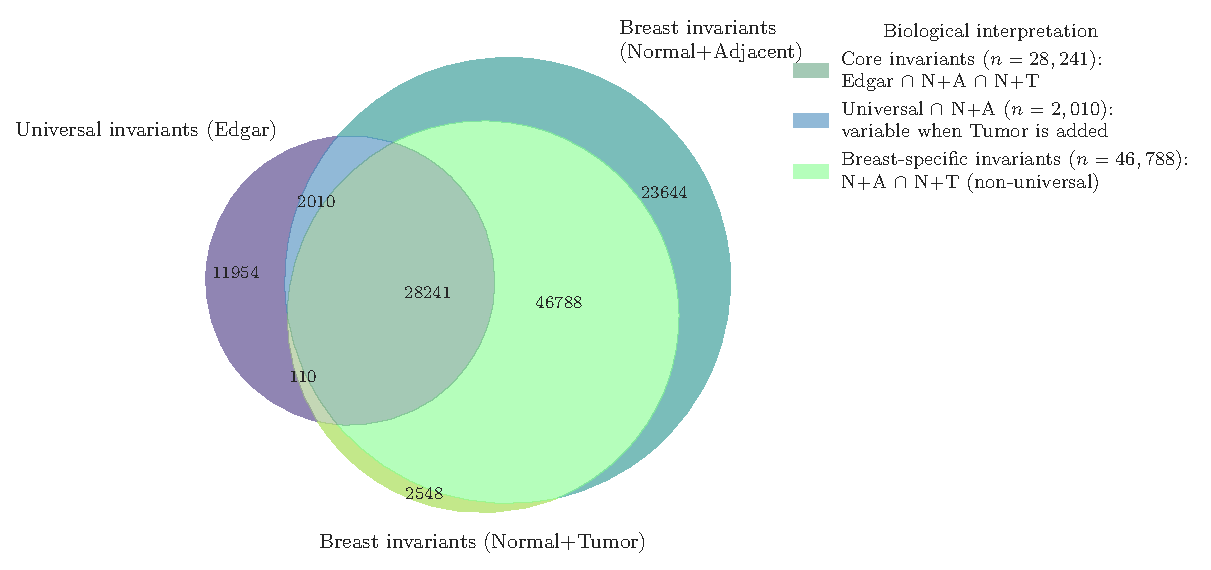
\includegraphics[width=\linewidth]{images/appendix/GSE69914_venn_universal_vs_NA_vs_NT}
        \caption{GSE69914}
        \label{fig:app_venn_69914}
    \end{subfigure}

    \vspace{0.5cm}

    % -------- (b) GSE225845 --------
    \begin{subfigure}{0.8\linewidth}
        \centering
        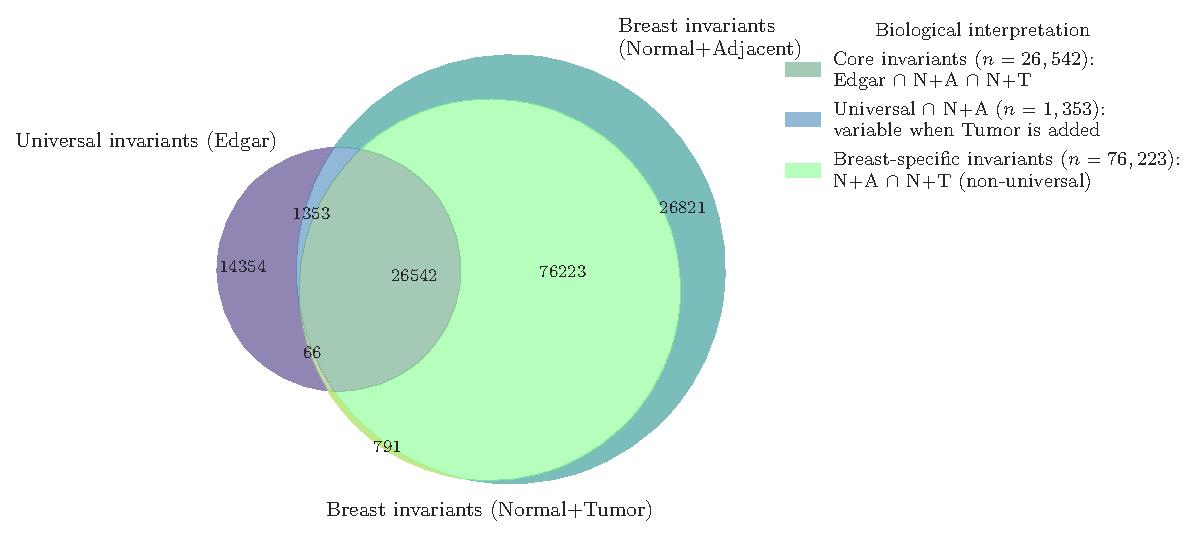
\includegraphics[width=\linewidth]{images/appendix/GSE225845_venn_universal_vs_NA_vs_NT}
        \caption{GSE225845}
        \label{fig:app_venn_225845}
    \end{subfigure}

    \vspace{0.5cm}

    % -------- (c) GSE287331 --------
    \begin{subfigure}{0.8\linewidth}
        \centering
        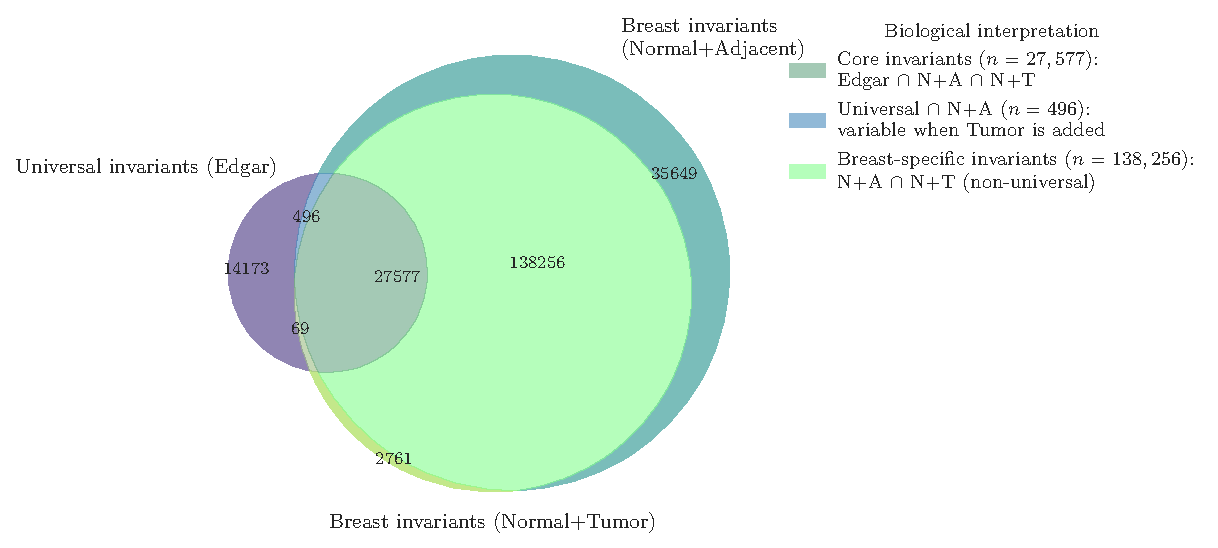
\includegraphics[width=\linewidth]{images/appendix/GSE287331_venn_universal_vs_NA_vs_NT}
        \caption{GSE287331}
        \label{fig:app_venn_287331}
    \end{subfigure}

    \caption{
    Overlap between universal invariants and 
    breast-specific invariant sets derived from the 
    Normal+Adjacent and Normal+Tumor contrasts in each dataset.
    }
    \label{fig:app_venn_universal_vs_breast}
\end{figure}